\section{Introduction}
A long-term goal of robotics research is the introduction of intelligent household robots.
To be effective, such robots will need to perform complex tasks
over long horizons (e.g., setting a dinner table, doing laundry). Planning for these long-horizon tasks is infeasible
for state-of-the-art motion planners, making the need
for a hierarchical system of reasoning apparent.

One way to approach hierarchical planning is through combined \emph{task and motion planning} (TAMP). In this
approach, an agent is given a symbolic, logical characterization of actions (e.g., move, grasp,
putdown), along with a geometric encoding of the environment.
TAMP systems maintain a hierarchical separation of high-level, symbolic task planning
and low-level, geometric motion planning.
Efficient integration of these two types of reasoning is challenging, and recent research has
proposed several methods for it~\cite{srivastava2014combined, kaelbling2011hierarchical,
lagriffoul2014orientation, GarrettWAFR14, dornhege2012semantic}.

\begin{figure}[t]
  \centering
    \noindent
    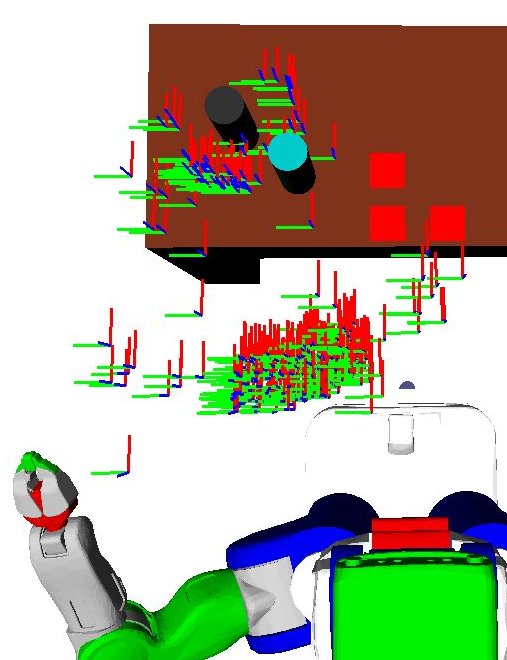
\includegraphics[scale=0.15]{images/move_grasp.png}\hspace{5 mm}
    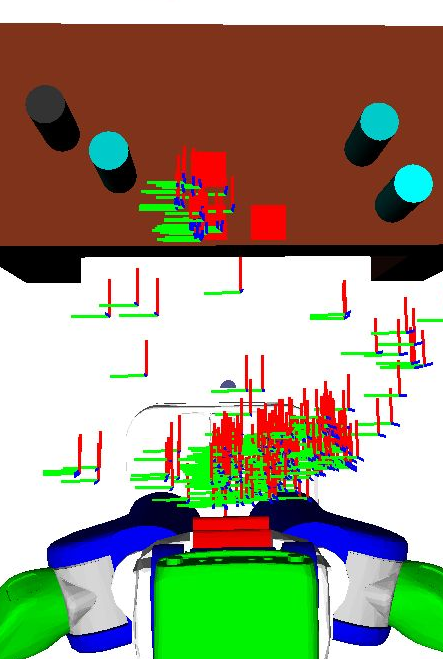
\includegraphics[scale=0.15]{images/move_putdown.png}
  \caption{\small{Screenshots showing distributions learned by our system in a simulated pick-and-place
    domain. We use reinforcement learning to train good sampling distributions for continuous motion
    planning parameters in long-horizon tasks. The robot must grasp the black can and put it down
    on the red square. The left image shows learned base position (blue) and grasping (green) distributions,
    and the right shows learned base position (blue) and putdown (green) distributions. The grasping policy
    learned to avoid the obstructions.}}
  \label{fig:cover}
  \vspace{-1.5 em}
\end{figure}

Our methods build on the TAMP system presented by Srivastava et al.~\cite{srivastava2014combined};
similar techniques could be applied for the TAMP approaches cited above. In Srivastava et al.,
a (classical) task planner produces a symbolic plan containing
a sequence of actions to reach a goal state. Then, in a process known as \emph{plan refinement},
candidate values are proposed for the continuous variables in this symbolic plan.
These values are checked locally for feasibility by calling a motion planner.
An advantage of this system is that the task planner and the motion planner are used as black boxes.

The authors propose an \emph{interface layer} for refining the plan into a set
of collision-free trajectories; it performs an exhaustive backtracking search over a
set of sampled candidate parameter values, which are instantiations of symbolic references in the plan. If a motion planning feasible
refinement is not found within the resource limit, symbolic error information is
propagated back to the task planner, and a new symbolic plan is produced.

The TAMP paradigms referenced above all use hand-coded heuristics to instantiate symbols with continuous values.
The system presented by Srivastava et al. relies on hand-coded discretizations to sample values for
plan parameters. Designing these heuristic sampling distributions often requires substantial effort.
They typically depend on geometric attributes of the environment and its objects and must be
re-calibrated to run the system in a new setting. Further,
the discretizations must be fairly coarse to allow reasonable search speeds, meaning they inherently lack
robustness to increased environmental complexity.

Reinforcement learning (RL) refers to the process of an agent learning a policy (a mapping from states to actions)
in its environment that maximizes rewards. Zhang and Dietterich~\cite{JobShopSched} first applied the RL framework
to planning problems, using a job shop scheduling setting. In this work, we take inspiration from
their approach; we use RL to train continuous proposal distributions for
plan refinement in a TAMP system. We implement our approach using methods adapted from
Zucker et al.~\cite{workspacebias}, who train a configuration space sampler for motion planning
using features of the discretized workspace.

Unpublished work that is currently in progress extends the system in~\cite{srivastava2014combined} to achieve completeness by
maintaining a \emph{plan refinement graph}, whose nodes each store a valid
symbolic plan (that reaches the goal) and its current parameter values. This makes it possible to interleave
partial refinement of several plans. In this paper, we also develop a method for making the decision of
which plan to try refining next.

The four contributions of our work are as follows: 1) we present randomized refinement, a local search
algorithm for plan refinement that is easily formulated as an MDP; 2) we formulate plan refinement in the
RL framework and learn a policy for this MDP; 3) we train heuristics to search intelligently
through a plan refinement graph, allowing us to decide which plan to try refining next;
and 4) we present experiments to evaluate our approach in a variety of simulated
domains. Our results demonstrate that our approach yields significantly improved
performance over that of hand-coded discretizations of the plan refinement sample space.
